\section{Durchführung}
\label{sec:Durchführung}

Für den Versuch wird der in \autoref{fig:messapparat} dargestellte Aufbau verwendet. Die Proben werden in einem, in \autoref{fig:therm} zu sehenden, Gefäß aktiviert und aufbewahrt.

\begin{figure}[H]
    \centering
    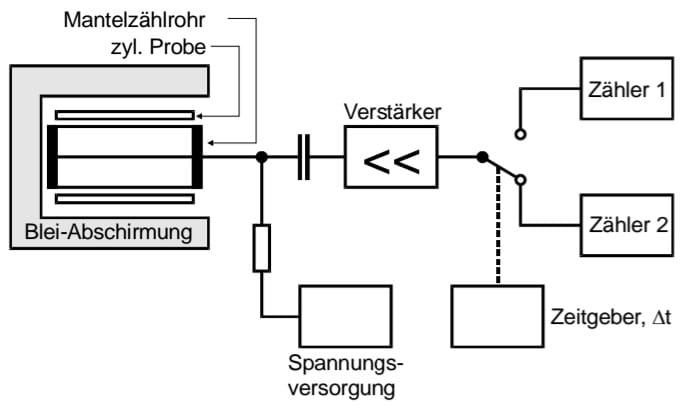
\includegraphics[width=\textwidth]{data/messapparat.jpeg}
    \caption{Schematische Darstellung des Versuchsaufbaus.}
    \label{fig:messapparat}
\end{figure}

Bevor die eigentlichen Messungen starten, muss zunächst eine Messreihe ohne Probe durchgeführt werden. Sie ist zur Bestimmung des Nulleffekts, also den Einflüssen
der natürlichen radioaktiven Strahlung, notwendig. Zur Bestimmung wird also eine relativ lange Messung von $t = \SI{600}{\second}$ durchgeführt. Die gemessene Anzahl
an Impulsen kann dann für spätere Messungen auf kürzere Intervalle runtergerechnet und abgezogen werden, um die von den Proben ausgehende radioaktive Strahlung möglichst
zu isolieren.\\
\newline
Für die erste Messreihe soll die Halbwertszeit von Vanadium untersucht werden. Das empfohlene Messintervall für Vanadium ist als $\SI{30}{\second}$ gegeben. Die
empfohlene Messzeit insgesamt als $\SI{15}{\minute}$. Es werden also 30 Messungen durchgeführt, die jeweils $\SI{30}{\second}$ lang sind.\\
Bei der zweiten Messreihe sollte wiederum die Halbwertszeit von Silber untersucht werden. Für Silber ist das empfohlene Messintervall $\SI{8}{\second}$ und die
empfohlene Messzeit insgesamt $\SI{7}{\minute}$. Mit der Silberprobe wurden also insgesamt 53 Messungen mit je $\SI{8}{\second}$ Messzeit durchgeführt.